\documentclass[11pt,titlepage]{article}

% Pretty much all of the ams maths packages
\usepackage{amsmath,amsthm,amssymb,amsfonts}

%page layout
\usepackage[margin=1in]{geometry}

% Removes paragraph indentation (not needed most of the time now)
\usepackage{parskip}
\usepackage{setspace}

% Allows inclusion of graphics easily and configurably
\usepackage{graphicx}

% Provides ways to make nice looking tables
\usepackage{booktabs}

% Allows you to rotate tables and figures
\usepackage{rotating}

\usepackage{titlesec}

%\usepackage{mathptmx}
\usepackage{chemfig}
\usepackage{tikz}
\usetikzlibrary{arrows,positioning,shapes.geometric,shapes.misc}

\usepackage{authblk}
\usepackage{wrapfig}

% Allows shading of table cells
\usepackage{colortbl}
% Define a simple command to use at the start of a table row to make it have a shaded background
\newcommand{\gray}{\rowcolor[gray]{.9}}

\usepackage{textcomp}

% Provides commands to make subfigures (figures with (a), (b) and (c))
\usepackage{subfigure}

% Typesets URLs sensibly - with tt font, clickable in PDFs, and not breaking across lines
\usepackage{url}

% Makes references hyperlinks in PDF output
\usepackage{hyperref}


% Provides good access to colours
\usepackage{color}
\usepackage{xcolor}

% Vastly improves the standard formatting of captions
\usepackage[margin=10pt,font=small,labelfont=bf, labelsep=endash]{caption}
\renewcommand{\baselinestretch}{1.5}

%\titleformat{\subsection}
%{\normalfont\itshape}{\thesubsection}{1em}{}

%opening
\title{A Novel Orientation-Dependent Potential for \\Protein Structure Prediction}
\author{Venkatesh Sivaraman}
%\author[2,3]{Eshel Faraggi}
%\author[3,4]{Andrzej Kloczkowski}
%\affil[1]{Bexley High School}
%\affil[2]{Indiana University School of Medicine}
%\affil[3]{Nationwide Children's Hospital}
%\affil[4]{The Ohio State University}

\begin{document}

\maketitle

\raggedbottom

\begin{abstract}
Protein structure prediction is one of the major unsolved problems in computational biology, primarily due to the inefficiency and short time scales of detailed simulations. We describe a novel statistical potential, called Segmented Positional Analysis of Residue Contacts (SPARC), which approximates the energy of a protein structure based on orientational inter-residue interactions as well as a packing density-like hydrophobicity term. Relative orientations are measured from a sample of 91,995 structures from the Protein Data Bank. The accuracy of SPARC is demonstrated first by comparison to CHARMM, a physics-based force field, and then to other statistical potentials on the gapless threading problem. SPARC showed an accuracy of 68\%, superior to a distance-dependent method and comparable to GOAP, an all-atom anisotropic potential.

In addition to the new statistical potential, a novel adaptation of the Metropolis-Hastings algorithm was designed for conducting Monte Carlo simulations of protein folding. The new method dynamically segments the protein into clusters to control variability and selects conformations with ``permissible'' orientations to ensure chain connectivity. We apply this algorithm to the structure prediction of bovine pancreatic trypsin inhibitor, yielding a structure with root mean square deviation of 8.78 \AA\, from the native structure after only 2,000 iterations. Together, SPARC and the new simulation technique will help biologists study the causes of protein folding disorders, model enzyme behavior, and engineer new proteins.
\end{abstract}

\section{Introduction}
Predicting the 3-dimensional structure of proteins remains a challenge despite advances in theory and computational power over the past three decades.
Modeling protein folding has numerous biological applications, including active site detection, protein design, and visualizing the formation of complexes, ligand binding, and protein-membrane interactions \cite{baker2,kouza,monticelli}.
However, the most detailed simulations must incorporate hundreds of atoms at picosecond time intervals, which currently prohibits the timescale on which these simulations can be computed.
Therefore, many biological applications would benefit from a coarse-grained approach that preserves as much detail as possible from atomistic methods.

The thermodynamic hypothesis, proposed by Anfinsen, stipulates that the native structure corresponds to the free energy minimum of all possible conformational states of the protein \cite{anfinsen}.
Therefore, the crux of structure prediction methods is to accurately express the energy of a protein in a given state. 
Energy functions generally fall under two categories: ``physics-based'' and ``knowledge-based potentials'' \cite{lu}.
Physics-based potentials and force fields, such as CHARMM \cite{brooks}, AMBER \cite{amber}, and GROMOS \cite{gromos}, evaluate conventional bonded and nonbonded energy terms (e.g. bond stretch, dihedral angle, and Coulombic potentials) for all atoms in a structure \cite{brooks2}.
These atomistic potentials can be made coarse-grained by modeling residues as one or a few particles, or by considering groups of residues as rigid subparts \cite{basdevant,potestio,enciso,monticelli}.
However, physics-based potentials necessitate either the inclusion of explicit solvent molecules in the simulation \cite{onufriev} or the use of implicit solvent techniques such as the generalized Born/solvent-accessible surface area (GBSA) model \cite{feig,roux}.
This tends to render all-atom force fields computationally inefficient if not intractable in large-scale molecular dynamics (MD) applications.

Knowledge-based potentials (KBPs) have developed as an approximative substitute for physics-based potentials and are more efficient at comparative tasks such as the gapless threading problem, which involves choosing the most likely native structure out of an ensemble of candidates \cite{thomas2}.
KBPs, also known as ``statistical potentials,'' are based on statistical analysis of known protein structures rather than distinct physical or chemical interactions. 
The use of KBPs was pioneered by Tanaka and Scheraga \cite{tanaka}, then Miyazawa and Jernigan \cite{miyazawa}, who estimated inter-residue interaction energies by counting contacts (pairs of residues located within a certain cut-off distance of each other) between types of amino acids in known protein structures.

The underlying assumption in assembling these statistical energy functions is that the known structures, obtained by X-ray crystallography or NMR, correspond to equilibrium states \cite{buchete2003}. 
As a consequence, the frequency of a local structure (e.g. a contact, distance, or relative orientation) can be related to its conformational energy according to the Boltzmann distribution.
This yields the following commonly-used expression for calculating energies by statistical analysis:

\begin{equation}
E(s) = -kT\ln{P(s)}
\label{boltzmann_device}
\end{equation}

where $s$ represents a local conformation, $k$ is Boltzmann's constant, $T$ is the temperature, and $P(s)$ is the probability of the state occurring in equilibrium \cite{sippl}.

Beyond contact potentials, various methods have also been developed based on the distribution of Euclidean distances between residues, such as DOPE \cite{shen}, DFIRE \cite{zhou}, GOAP \cite{zhou2}, and others \cite{lu,zhang}.
A few studies have incorporated anisotropic factors by comparing the orientations of the sidechains \cite{zhang3,mukherjee} or by measuring polar, spherical and/or Euler angles between two contacting residues \cite{miyazawa2,buchete2003}. 
In general orientation-dependent energy terms based on bond angles are also combined with dedicated distance-dependent components, though the additivity of these conceptually distinct quantities has been questioned \cite{shen}.
Moreover, these statistical potentials may be limited by their concern with only the backbone or the sidechains, as well as failure to consider the tendency of hydrophobic residues to move toward the protein core \cite{mullinax}.

This paper presents a new anisotropic statistical potential, called Segmented Positional Analysis of Residue Contacts (SPARC), that addresses concerns with other statistical methods by generalizing the expression of amino acid orientations through local coordinate system transformations.
We describe the methods used to derive SPARC from the database of known protein structures, as well as a ``coordination number''-based implicit solvent interaction model.
SPARC is then evaluated based on its performance on the gapless threading problem in comparison to other statistical potentials, and tested in a new segmented dynamic Monte Carlo simulation of protein folding.

\section{Methods}

\begin{figure}
	\begin{center}
		\begin{tikzpicture}
		\setbondoffset{3pt}
		\draw[->,>=stealth] (0.2,0) -- (2.5,0) node [right,black] {\textbf{j}};
		\draw (-0.5,0) -- (-2.5,0);
		\draw[->,>=stealth] (0,2.1) -- (0,2.5) node [above,black] {\textbf{k}};
		\draw (0,-0.4) -- (0,-2.3);
		\draw[->,>=stealth] (-0.3,-0.3) -- (-1.8,-1.8);
		\node at (-2, -2) {\textbf{i}};
		\draw (0.2,0.2) -- (1.7,1.7);
		\node at (0,0) {\chemfig[][scale=1.6]{C_\alpha(-[2]R)(<[:240]H)(>:[:340]C)(>:[:200]N)}};
		\end{tikzpicture}
	\end{center}
	\caption{The core structure of an amino acid around the $\alpha$-carbon. We utilize the bond angles predicted by VSEPR theory to assign each amino acid a local coordinate system.}
	\label{aminoacid_axes}
\end{figure}

\subsection{Construction of local coordinate system}
Given a protein $A$ of $n$ amino acids, we can assign a Cartesian local coordinate system (LCS) to each residue to quantify its orientation with respect to an arbitrary global coordinate system (GCS).
To determine a set of basis vectors that is consistent across all 20 sidechain types, we turn to the ideal bond angles predicted by valence-shell electron-pair repulsion (VSEPR) theory \cite{gillespie}.
As shown in Fig. \ref{aminoacid_axes}, the bond geometry around the C$_\alpha$ atom is approximately tetrahedral, with bond angles of $\cos^{-1}{-1/3}\approx 109.5^\circ$.

Defining $\textbf{n}$ and $\textbf{c}$ as the normalized vectors in the GCS pointing from C$_\alpha$ to the amine nitrogen and carbonyl carbon, respectively, we define $\textbf{j} \equiv \pm(\textbf{n} - \textbf{c})$, with the sign that minimizes the angle between \textbf{j} and \textbf{c}.
We proceed with the \textbf{k} vector, which should lie along the bond leading to the sidechain (or a hydrogen atom in the case of glycine).
Solving for a unit vector \textbf{k} from its bond angles with \textbf{c} and \textbf{n},

\begin{align*}
\textbf{n}\cdot\textbf{k} &= -1/3
\\ \textbf{c}\cdot\textbf{k} &= -1/3
\end{align*}

we obtain two solutions, each of which has an associated vector $\textbf{i}=\textbf{j}\times\textbf{k}$.
The pair that maximizes the angle between \textbf{i} and \textbf{c} produces an LCS consistent with Fig. \ref{aminoacid_axes}.

\subsection{From orientational frequencies to energies}
The Cartesian LCS for each amino acid enables us to describe the relative orientation between any two amino acids $\textbf{p}$ and $\textbf{q}$ as simply the coordinates of $\textbf{p}$ in the LCS of $\textbf{q}$, denoted $\textbf{p}_q$, and vice versa.
To obtain a distribution of relative orientations for each sidechain type, we consider only those amino acids within a contact sphere of radius 10 \AA\, of each residue, a set we denote $A^*$.
The orientation space is coarse-grained into intervals of 1 \AA\, for a total of 8,000 possible ``bins'' into which each relative location might fall. (Because the contact shell is spherical and contained within a rectangular orientation space, in reality only about 4,200 bins would be used.)

As in all statistical potentials, SPARC assumes that these pairwise orientations are Boltzmann-distributed in an ensemble of native protein structures \cite{sippl}, motivated by the fact that even at a global energy minimum, unstable \textit{local} structures can still be found.
This permits us to adapt Eq. (\ref{boltzmann_device}) to calculate a dimensionless energylike quantity from the orientational frequencies:
\begin{equation}
\displaystyle
S(\textbf{p}) = -\sum_{\textbf{q}\in A_p^*} \left(\ln{\frac{f(\textbf{p}_q)f_{pq,\text{tot}}}{\bar{f}_{pq}\bar{f}_\text{tot}}} + \ln{\frac{f(\textbf{q}_p)f_{pq,\text{tot}}}{\bar{f}_{pq}\bar{f}_\text{tot}}}\right)
\label{sparc_equation}
\end{equation}
In this equation, which sums over all amino acids within the contact sphere $A_p^*$, $f(\textbf{p}_q)$ refers to the frequency of an interaction between amino acids of type $p$ and $q$ with that particular relative location. 
$\bar{f}_{pq}$ represents the mean frequency over all bins, and $f_{pq,\text{tot}}$ the total number of contacts for these amino acid types (e.g. alanine and tyrosine, glycine and glutamine, etc.).
$\bar{f}_\text{tot}$ is the mean number of contacts over all combinations of amino acid types.
The result of this formulation is that contacts whose relative orientations are above average receive a more negative (stable) score.
Furthermore, for a perfectly ``average'' orientation, a more negative score will result if contacts between amino acid types $p$ and $q$ are more frequent in the native ensemble.

Another important consideration when constructing SPARC was chain connectivity, since amino acids adjacent to each other along the peptide backbone interact differently (due to the presence of connecting covalent bonds) than non-consecutive residues.
Therefore, the consecutive and non-consecutive amino acids found within the 10-\AA\, shell were separated and analyzed separately, producing two distinct score functions $S_c$ and $S_{nc}$.

\subsection{Solvent interaction model}
In an implicit solvent, the intermolecular interactions that determine the stability of a protein structure can be decomposed into residue-residue and residue-solvent interactions.
The latter cannot be modeled by orientation in an implicit solvent, so they are collectively modeled by SPARC in terms of the ``coordination number'' or packing density of the residues.
This approximation is similar to the coordination numbers used by Miyazawa and Jernigan \cite{miyazawa}; however, instead of calculating the values indirectly from the volume of each residue type, we count the number of amino acids within the contact sphere (see section \ref{materials}).
The analog for Eq. (\ref{sparc_equation}) for the solvent interactions then becomes

\begin{equation}
S_{\text{solv}}(\textbf{p}) = -\ln{\frac{f(|A_p^*|)}{\bar{f}_p}},
\label{solvent_equation}
\end{equation}

where $\bar{f}_p$ is the mean frequency over the possible coordination numbers for amino acid type $p$.
The energylike quantities represented by $S_c$, $S_{nc}$, and $S_\text{solv}$ are finally combined linearly to produce an overall SPARC score value.

\subsection{Dynamic Monte Carlo simulation}
\begin{figure}
	\begin{center}
		\setstretch{1.0}
		\small
		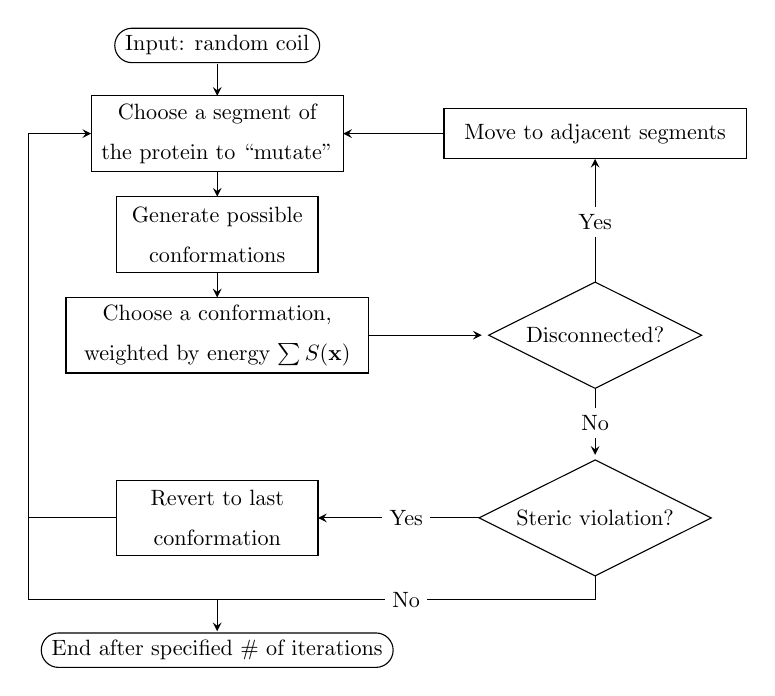
\begin{tikzpicture}[scale=0.8, every node/.style={scale=0.8}]
		\draw [->, >=stealth] (0,-1.5) -- (0, -2);
		\draw [->, >=stealth] (0,-2.5) -- (0, -3.6);
		\draw [->, >=stealth] (0,-4.5) -- (0, -5.2);
		\draw [->, >=stealth] (0,-5.8) -- (4.2, -5.8);
		\draw [->, >=stealth] (6, -5.8) -- (6, -3);
		\draw [->, >=stealth] (3.6, -2.6) -- (2, -2.6);
		\draw [->, >=stealth] (6, -6.6) -- (6, -7.7);
		\draw [->, >=stealth] (6, -8.7) -- (1.6, -8.7);
		\draw (6, -8.7) -- (6, -10) --(-3, -10)  -- (-3, -8.7);
		\draw [->, >=stealth] (0, -8.7) -- (-3, -8.7) -- (-3, -2.6) -- (-2, -2.6);
		\draw [->, >=stealth] (0, -10) -- (0, -10.5);
		
		\node [draw, rounded rectangle, fill=white] at (0, -1.2) {Input: random coil};
		\draw [fill=white,text width=3.8cm,align=center] (-2,-2) rectangle (2,-3.2) node[pos=.5] {Choose a segment of the protein to ``mutate''};
		\draw [fill=white,text width=3cm,align=center] (-1.6,-3.6) rectangle (1.6,-4.8) node[pos=.5] {Generate possible conformations};
		\draw [fill=white,text width=4.5cm,align=center] (-2.4,-5.2) rectangle (2.4,-6.4) node[pos=.5] {Choose a conformation, weighted by energy $\sum S(\textbf{x})$};
		\node [draw, diamond, fill=white, aspect=2] at (6, -5.8) {Disconnected?};
		\node [fill, white, rectangle, text=black] at (6, -4) {Yes};
		\node [fill, white, rectangle, text=black] at (6, -7.2) {No};
		\node [draw, diamond, fill=white, aspect=2] at (6, -8.7) {Steric violation?};
		\draw [fill=white,text width=4.4cm,align=center] (3.6,-2.2) rectangle (8.4,-3) node[pos=.5] {Move to adjacent segments};
		\node [fill, white, rectangle, text=black] at (3, -8.7) {Yes};
		\node [fill, white, rectangle, text=black] at (3, -10) {No};
		\draw [fill=white,text width=3cm,align=center] (-1.6,-8.1) rectangle (1.6,-9.3) node[pos=.5] {Revert to last conformation};
		\node [draw, rounded rectangle, fill=white] at (0, -10.8) {End after specified \# of iterations};
		\end{tikzpicture}
	\end{center}
	\caption{An overview of a Markov chain Monte Carlo (MCMC) simulation algorithm developed using SPARC. The procedure is similar to that of the Metropolis-Hastings algorithm in that new structures are sampled so that better-scoring conformations are chosen more often.}
	\label{flowchart}
\end{figure}
The statistical nature of SPARC makes it especially conducive to a Markov chain Monte Carlo (MCMC) simulation because it provides direct local stability comparisons which can be used to sample the conformational space.
Monte Carlo simulations have been used with some frequency to predict protein structure \cite{kolinski,enciso}, though not as often or as successfully as deterministic molecular dynamics (MD).
The most widely-used MCMC technique is the Metropolis-Hastings algorithm, which uses a weighted form of rejection sampling to approximate a distribution over a large number of iterations \cite{metropolis}.
We implement a modified version of the Metropolis-Hastings algorithm based on the distribution of relative orientations in SPARC, which should improve the speed and viability of Monte Carlo methods for protein structure prediction.

An overview of the simulation algorithm is presented in Fig. \ref{flowchart}.
During each iteration, segments of length $\ell$ are chosen at random, where $\ell$ is an initial parameter.
The SPARC scores of each possible ``mutation'' to the chosen segment can be transformed into probabilities:

\begin{equation}
P(C) = \exp{\left(-\sum_{\textbf{a}_i\in C}S(\textbf{a}_i)\right)}
\label{probability_eq}
\end{equation}

A cumulative distribution function is then obtained from the normalized values of $P(C)$, and sampled to determine the next local conformation.

To maintain chain connectivity, two additional modifications to the Metropolis-Hastings approach are necessary. 
First, the locations of consecutive residues are constrained to ``permissible'' orientations, which are found with at least a certain frequency (0.5\%) in the native ensemble; this ensures that the bonding between residues is realistic.
Second, the neighboring segments of the protein are adjusted to amend the breaks caused by each mutation.

\subsection{Materials and software}
\label{materials}
All calculations and programs were run on an off-the-shelf laptop computer and a desktop.
Written in Python 2.7 and comprising about 6,000 lines of code, this first version of the SPARC software contains tools for reading and writing PDB files, analyzing structures for orientation data directly from the Protein Data Bank, and running the dynamic Monte Carlo simulations as well as other utilities, with all modules designed to be subclassable and extendible for future modifications.

To calculate the orientational frequencies, a large dataset of native protein structures determined using X-ray crystallography (91,995 total structures) was obtained from the Protein Data Bank.
When performing relative orientation calculations, a hash table is utilized to map the amino acids into spatial ``buckets'' of dimension 5 \AA\, based on the location of the $\alpha$-carbon.
This results in a major performance improvement over searching the entire protein conformation for pairwise contacts, from $O(n)$ for each calculation to $O(1)$.

\section{Results}
\subsection{Frequency distributions}
\begin{figure}
	\begin{center}
		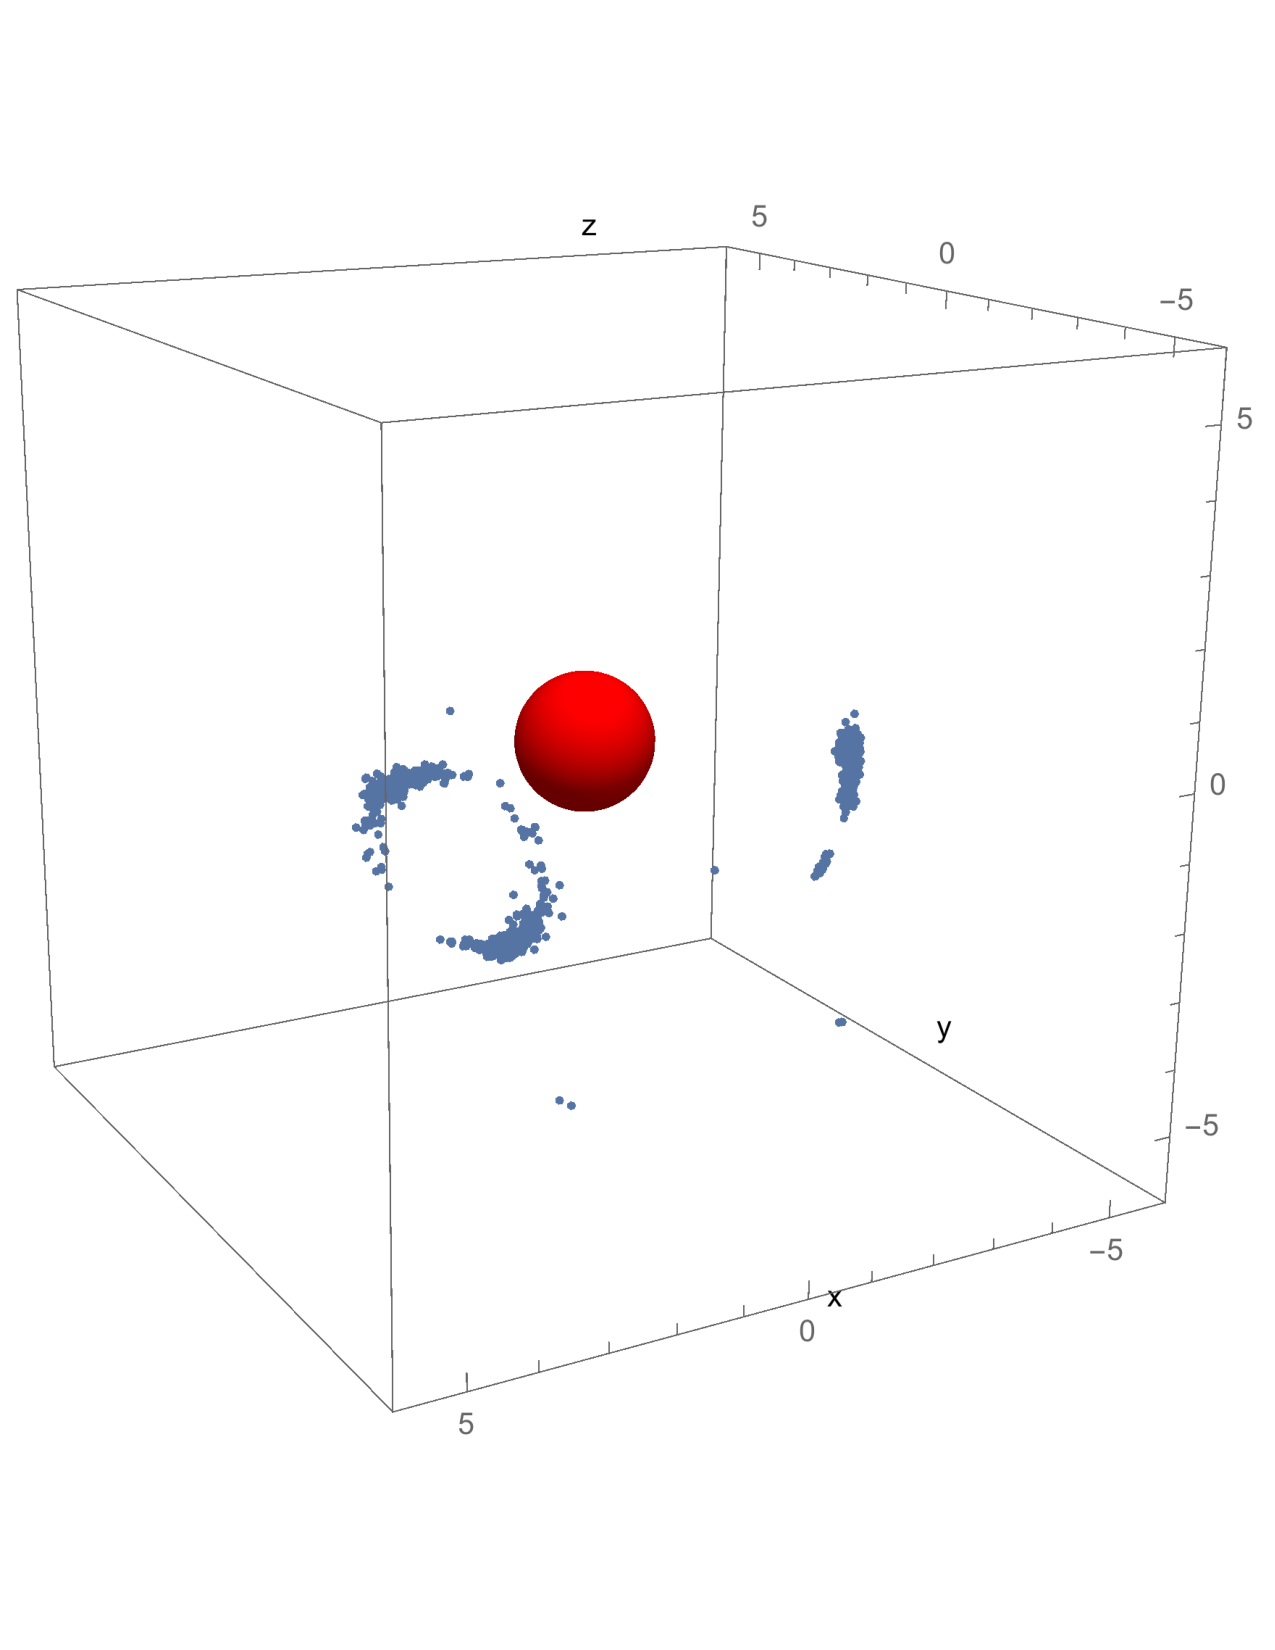
\includegraphics[trim={0 3cm 0 3cm}, clip=true, width=0.45\textwidth]{consec_alpha_frequencies}\,\,\,\,\,
		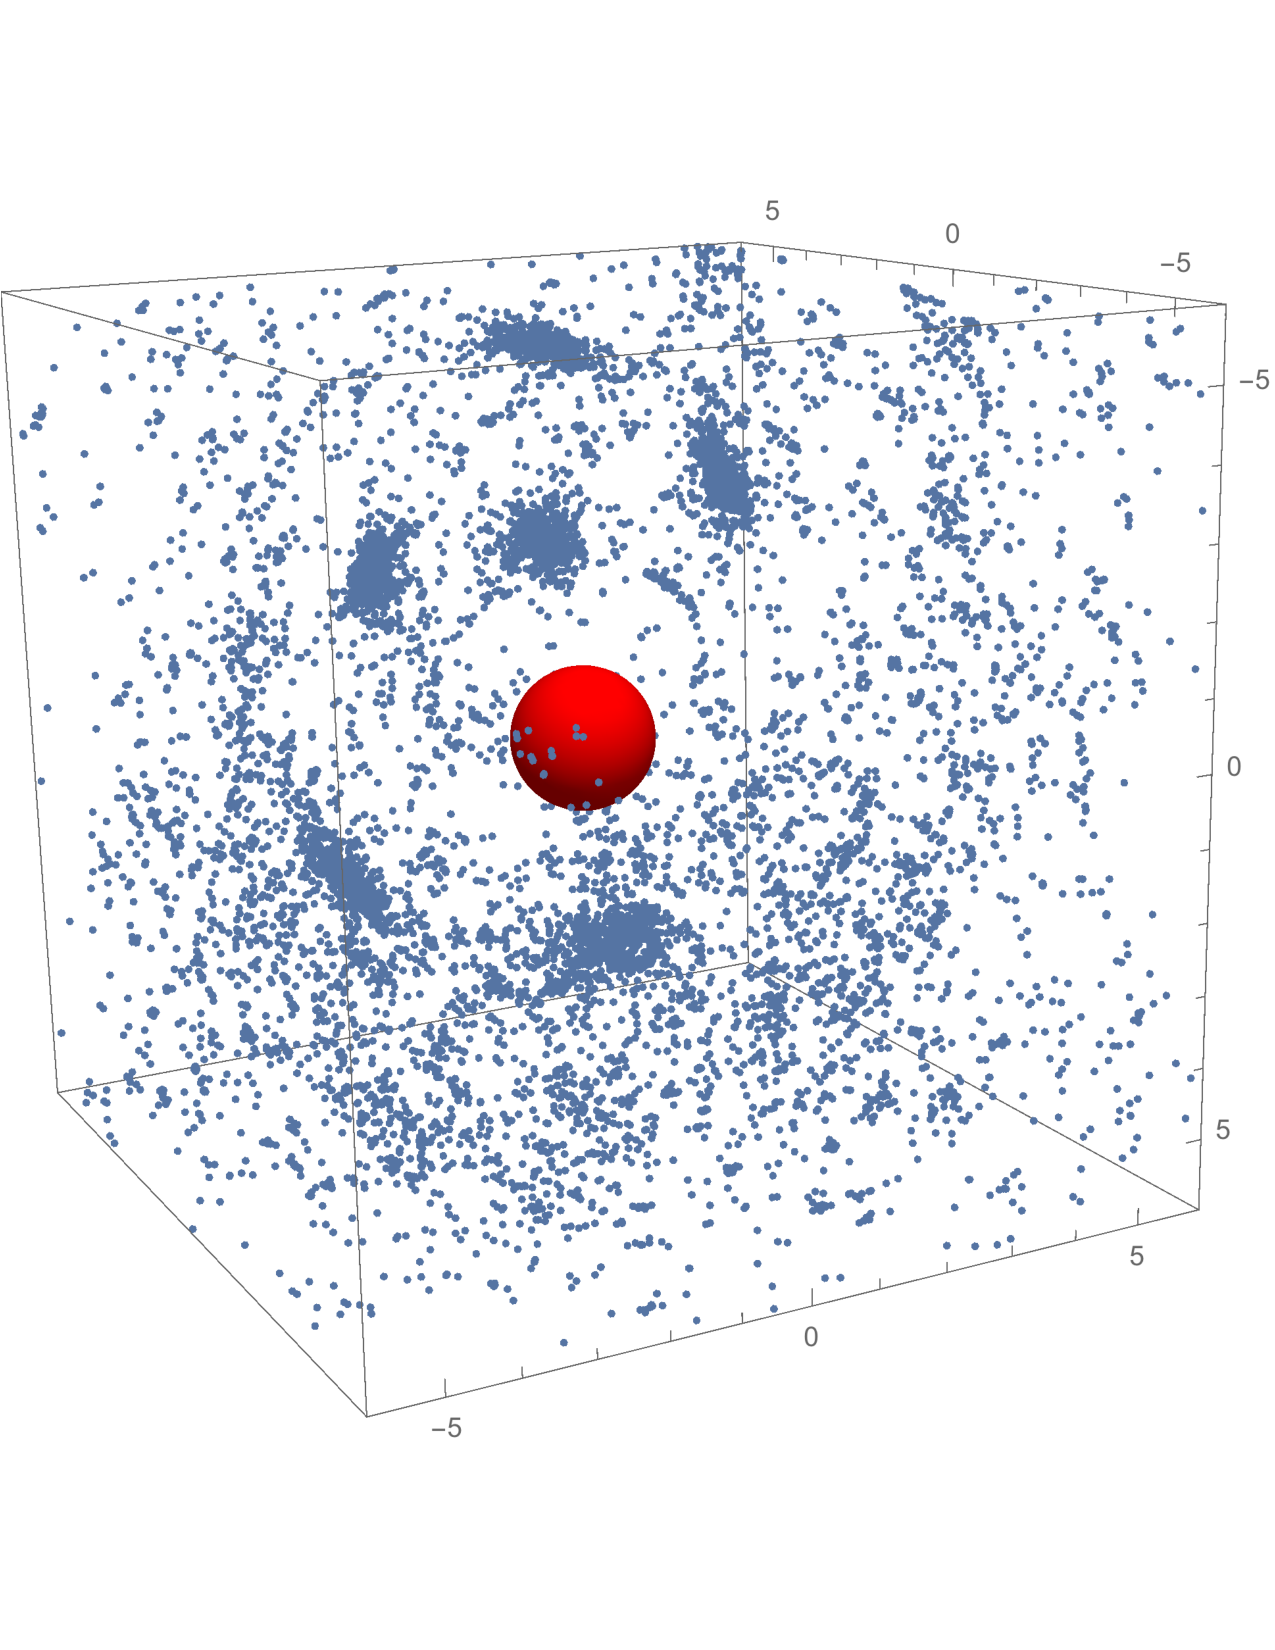
\includegraphics[trim={0 3cm 0 3cm}, clip=true, width=0.45\textwidth]{nonconsec_alpha_frequencies}
		\caption{A portion of the distribution of C$_\alpha$ relative locations between two alanine residues, consecutive (left) and non-consecutive (right). The consecutive distribution is much more specific due to the constraints imposed by peptide bond, while the nonconsecutive distribution permits many more possible locations.}
		\label{alpha_frequencies}
	\end{center}
\end{figure}
The large sample size of proteins used to construct SPARC allowed us to establish fairly small bins without considerable loss in accuracy.
For consecutive amino acids, it was expected that the vast majority of relative orientations would be located in a small number of bins, corresponding to the allowed angles of the peptide bond; this hypothesis was confirmed in Fig. \ref{alpha_frequencies}, left.
On average, 505 bins were filled and only 27 contained more than 50 occurrences.
The nonconsecutive distributions showed much more variability, also as expected because of the lack of a restrictive covalent bond (Fig. \ref{alpha_frequencies}, right): 4,032 bins were non-empty, almost all of the {\raisetag{.17ex\hbox{$\scriptstyle\sim$}}}4,200 possible bins.

While other techniques we attempted (orientations with respect to nearby residues, distance to the geometric center of the protein) failed to capture hydrophobicity sufficiently, the coordination-number approach does seem to accurately reflect the conventional hydrophobicity scale reported by Kyte and Doolittle \cite{kyte}.
Fig. \ref{hydrophobicities} illustrates the distributions of coordination numbers or packing densities around each amino acid type.
Nonpolar residues such as Ile and Val, the red curves, show a clear preference for a greater packing density (both Ile and Val had 21 residues within the contact shell on average).
Overall, the mean coordination numbers agreed with the Kyte-Doolittle ranking scale with a correlation coefficient $R^2=0.75$, as depicted in Fig. \ref{hydrophobicity_corr}. 
The main exceptions to this correlation were Trp and Tyr, which appeared more hydrophobic on the SPARC scale than they are conventionally described, and three of the charged amino acids (Lys, Asp, and Glu), which appeared more hydrophilic.
Regardless of the relative magnitudes of the means, the distributions proved useful in the simulation because the energy with respect to polarity of a specific residue could be easily approximated according to the coordination number distribution for its sidechain type.

\begin{figure}
	\begin{center}
	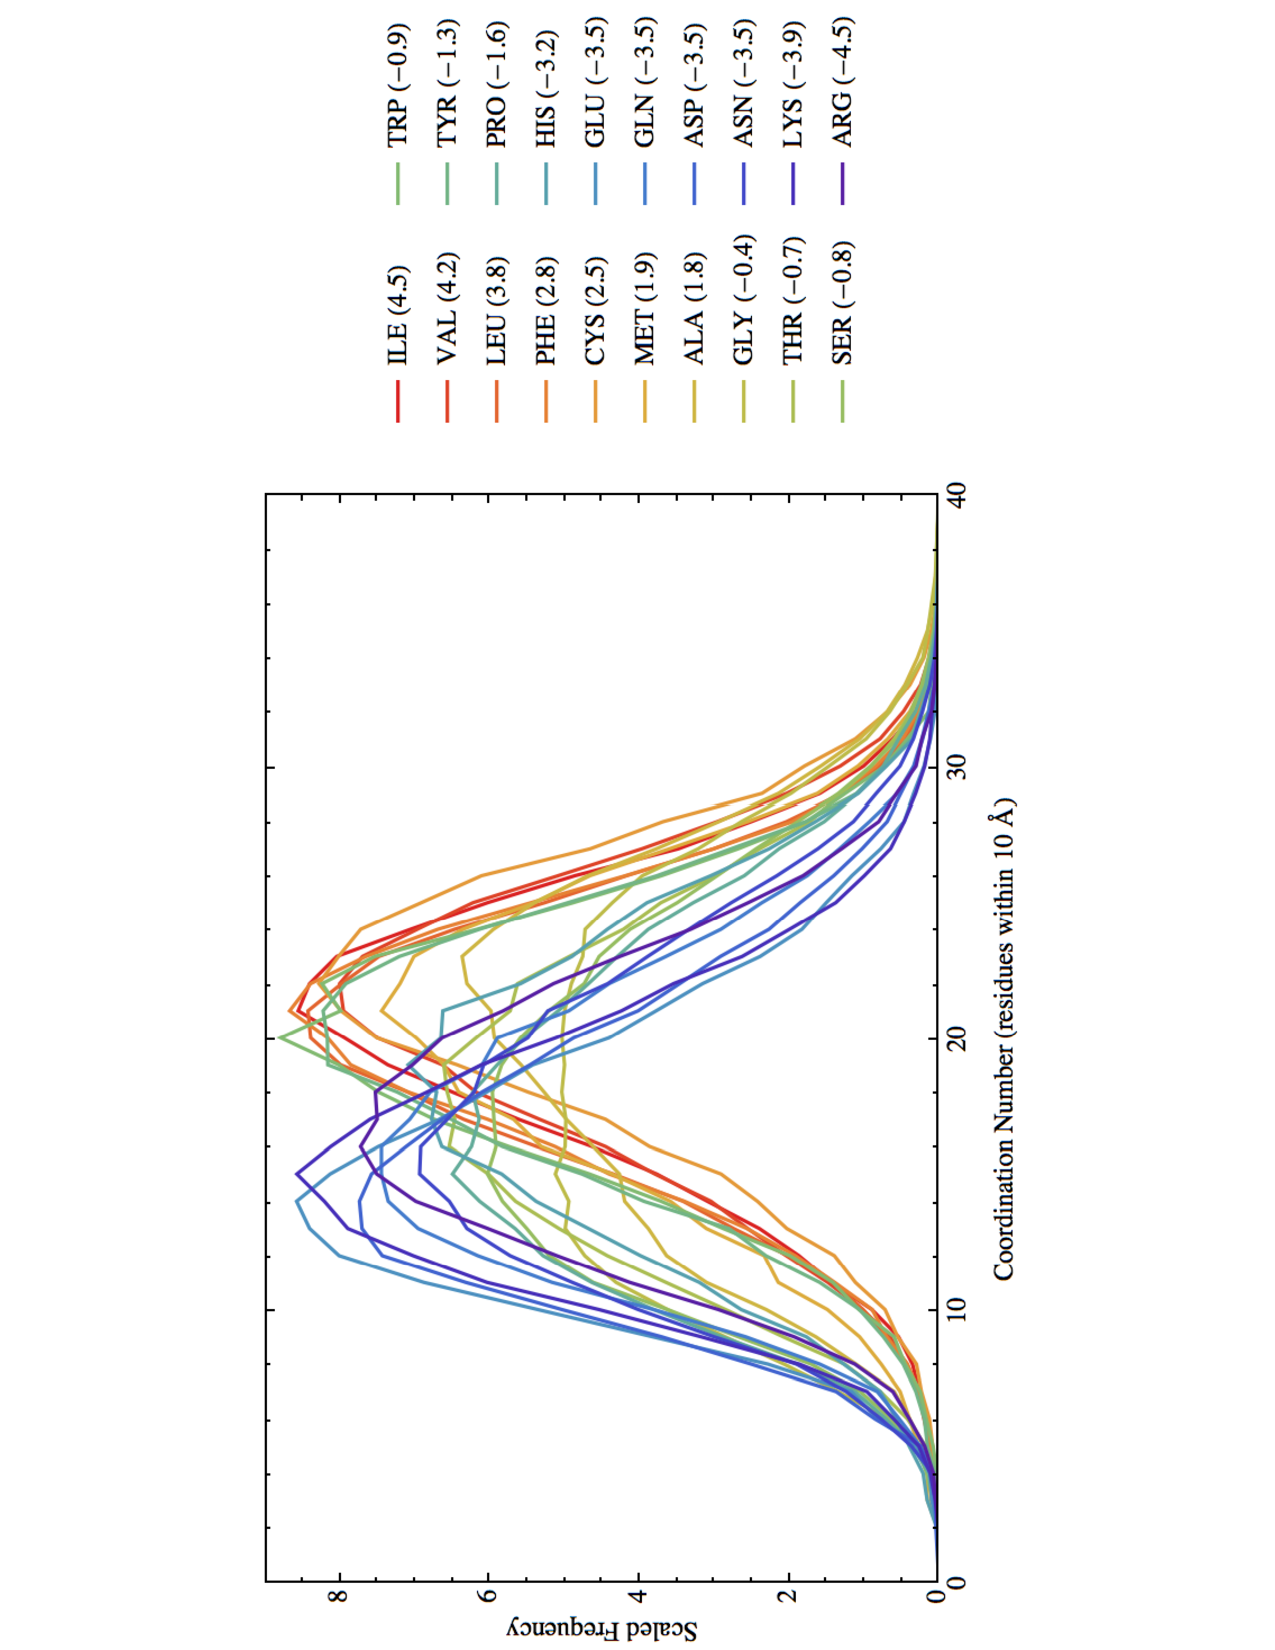
\includegraphics[trim={4cm 0cm 4cm 0cm}, height=0.8\textwidth,angle=-90]{hydrophobicity_graph}
	\end{center}
	\caption{The distributions of coordination numbers of each amino acid type, scaled from 1--10. The Kyte-Doolittle hydrophobicity values are given in parentheses; the blue hues are more polar residue types, and the red hues are more nonpolar.}
	\label{hydrophobicities}
\end{figure}


\begin{figure}
	\begin{center}
		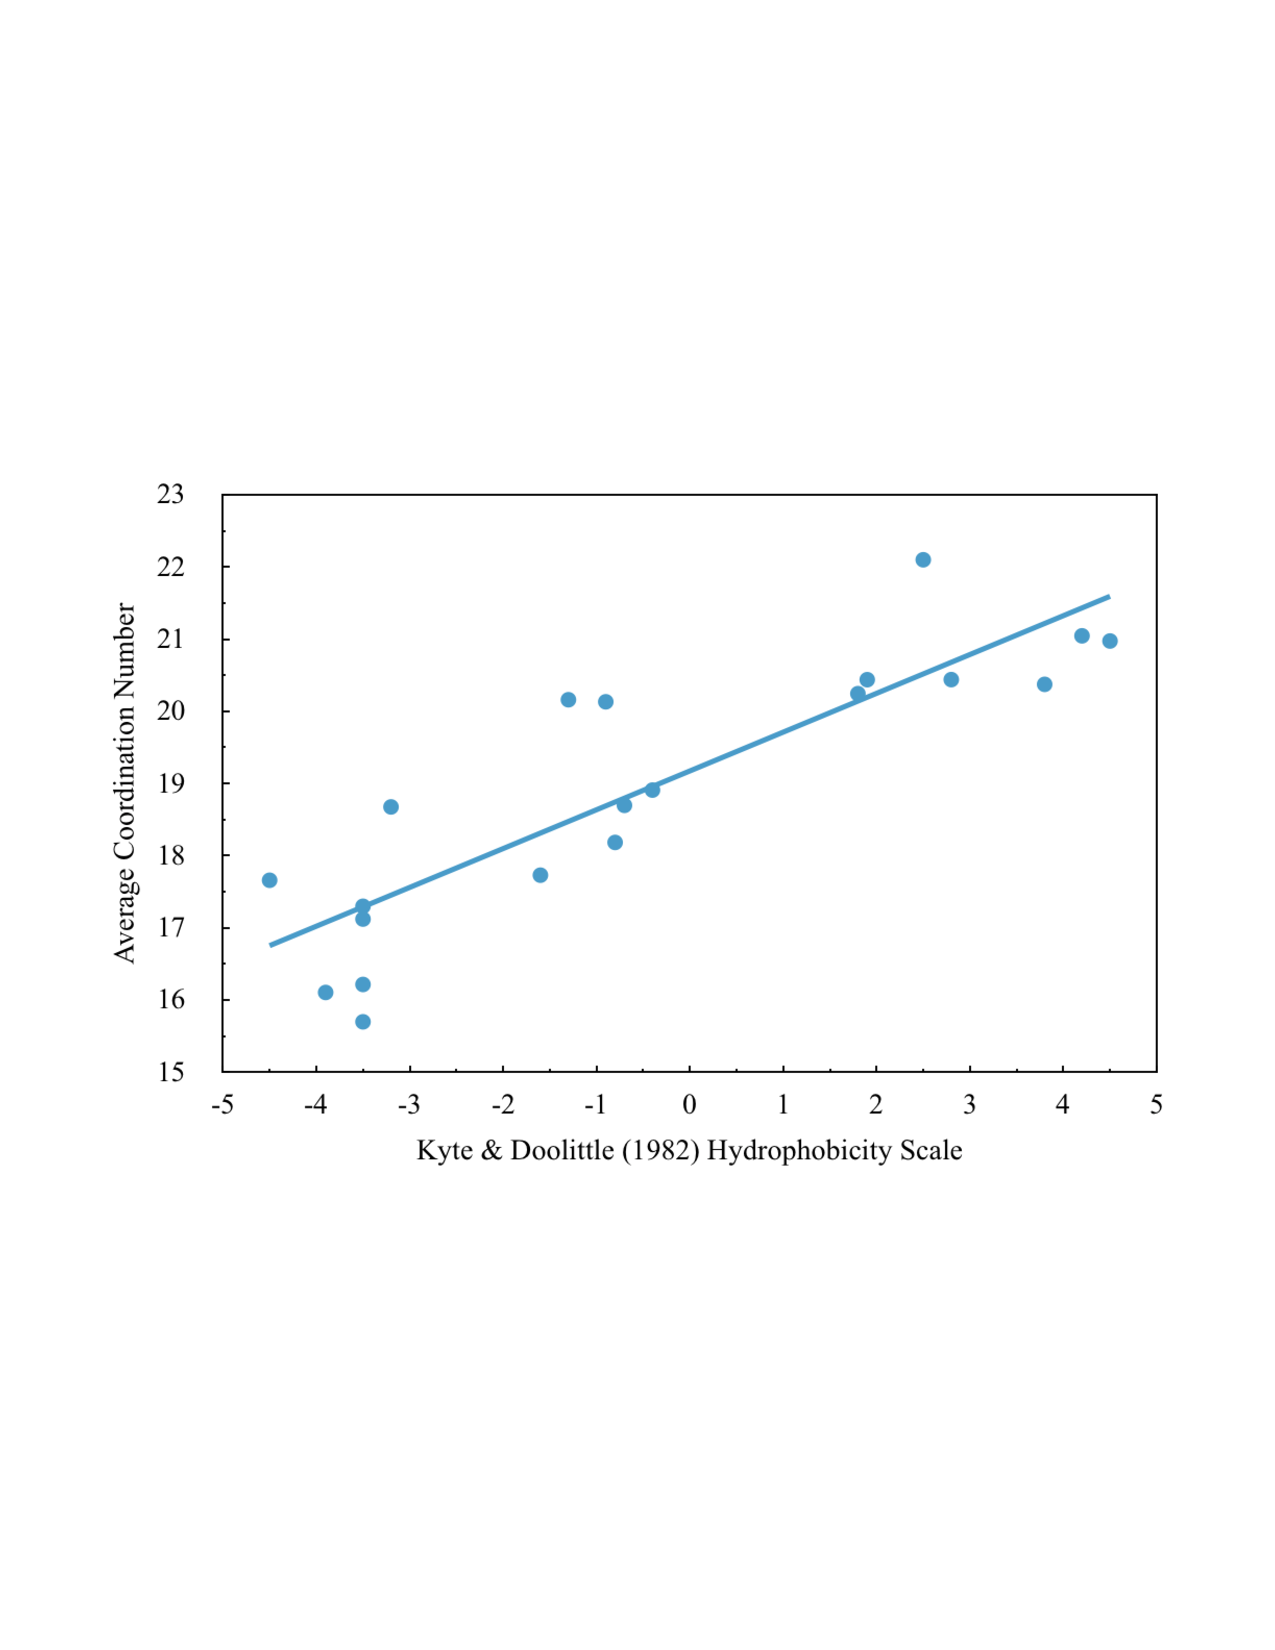
\includegraphics[trim=1cm 8cm 1cm 8cm, width=0.7\textwidth,keepaspectratio]{hydrophobicity_correlation}
	\end{center}
	\caption{A comparison of the Kyte and Doolittle hydrophobicity scale and the SPARC coordination number approach illustrates the correlation ($R^2=0.75$) between the packing density of residues within the structure and their polarity.}
	\label{hydrophobicity_corr}
\end{figure}

\subsection{Validation with CHARMM}

\begin{wrapfigure}{r}{0.4\textwidth}
	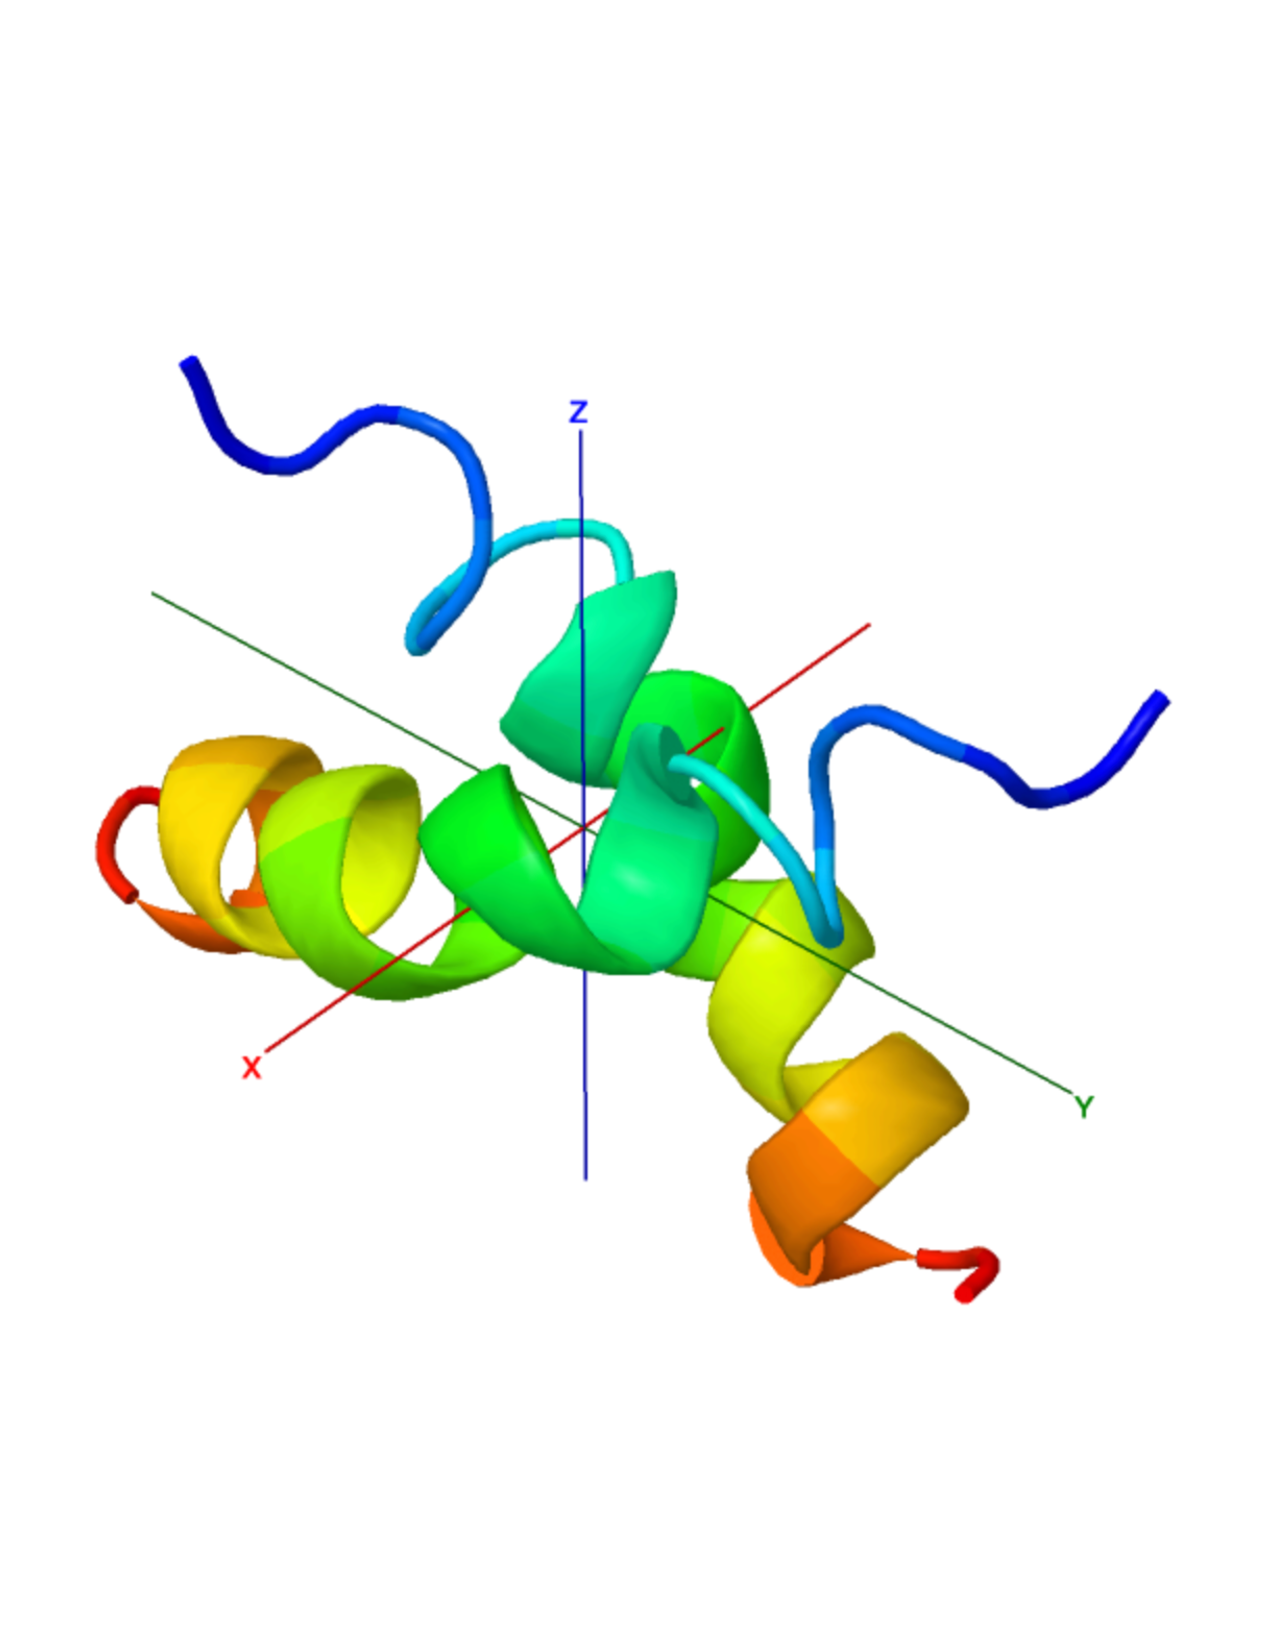
\includegraphics[trim={0 5cm 0 5cm}, clip=true, width=0.4\textwidth]{magainin_structure}
	\caption{The structure of magainin, a small antimicrobial protein. The distance between the two chains is varied to compare the scores yielded by CHARMM and SPARC.}
	\label{magainin}
\end{wrapfigure}

The correlation between knowledge-based potentials (KBPs) and all-atom force fields such as CHARMM is often tenuous because of the thermodynamic assumptions that are made on the native ensemble \cite{mullinax}, although some reports have demonstrated good correlations between the force fields and their potentials \cite{mohanty,basdevant}.
While SPARC is constructed on similar principles to many other KBPs, we hypothesized that because of the combination of the orientation-based residue interaction model and a solvent interaction term, it would correlate closely with the detailed all-atom potentials.
This was tested with a procedure similar to that used by Basdevant et al. \cite{basdevant}, based on the structure of the small antimicrobial protein magainin (PDB code 1DUM).
The magainin structure consists of two antiparallel $\alpha$-helices, as shown in Fig. \ref{magainin}.
The B-chain was translated incrementally in both the $xy$ and the $yz$ directions; for each distance, the SPARC inter-residue scores were calculated as well as the all-atom potentials using the CHARMM27 force field \textit{in vacuo} in the GROMACS command-line tool \cite{gromacs}.
The structures were relaxed first using a short MD simulation to prevent extremely high CHARMM energy values.

The comparison revealed an interesting relationship between the CHARMM and SPARC potential values.
As shown in Fig. \ref{magainin_graphs}, the SPARC score mimics the contours of the logarithm of the physics-based potential, especially in the $xy$-direction.
The large jump in the $xy$ graph, which occurs at around 15 \AA, is probably due to a steric clash and is exactly captured by SPARC; other blips are also evident in both curves.
However, the energy values do not strongly correlate with each other without the inclusion of the distance factor ($R^2=0.29$). 
This could be due to a lack of resolution in unstable structures, which obviously were not prevalent in the native ensemble used to construct our potential; SPARC would therefore be most useful for local comparisons between similar structures.

\begin{figure}
	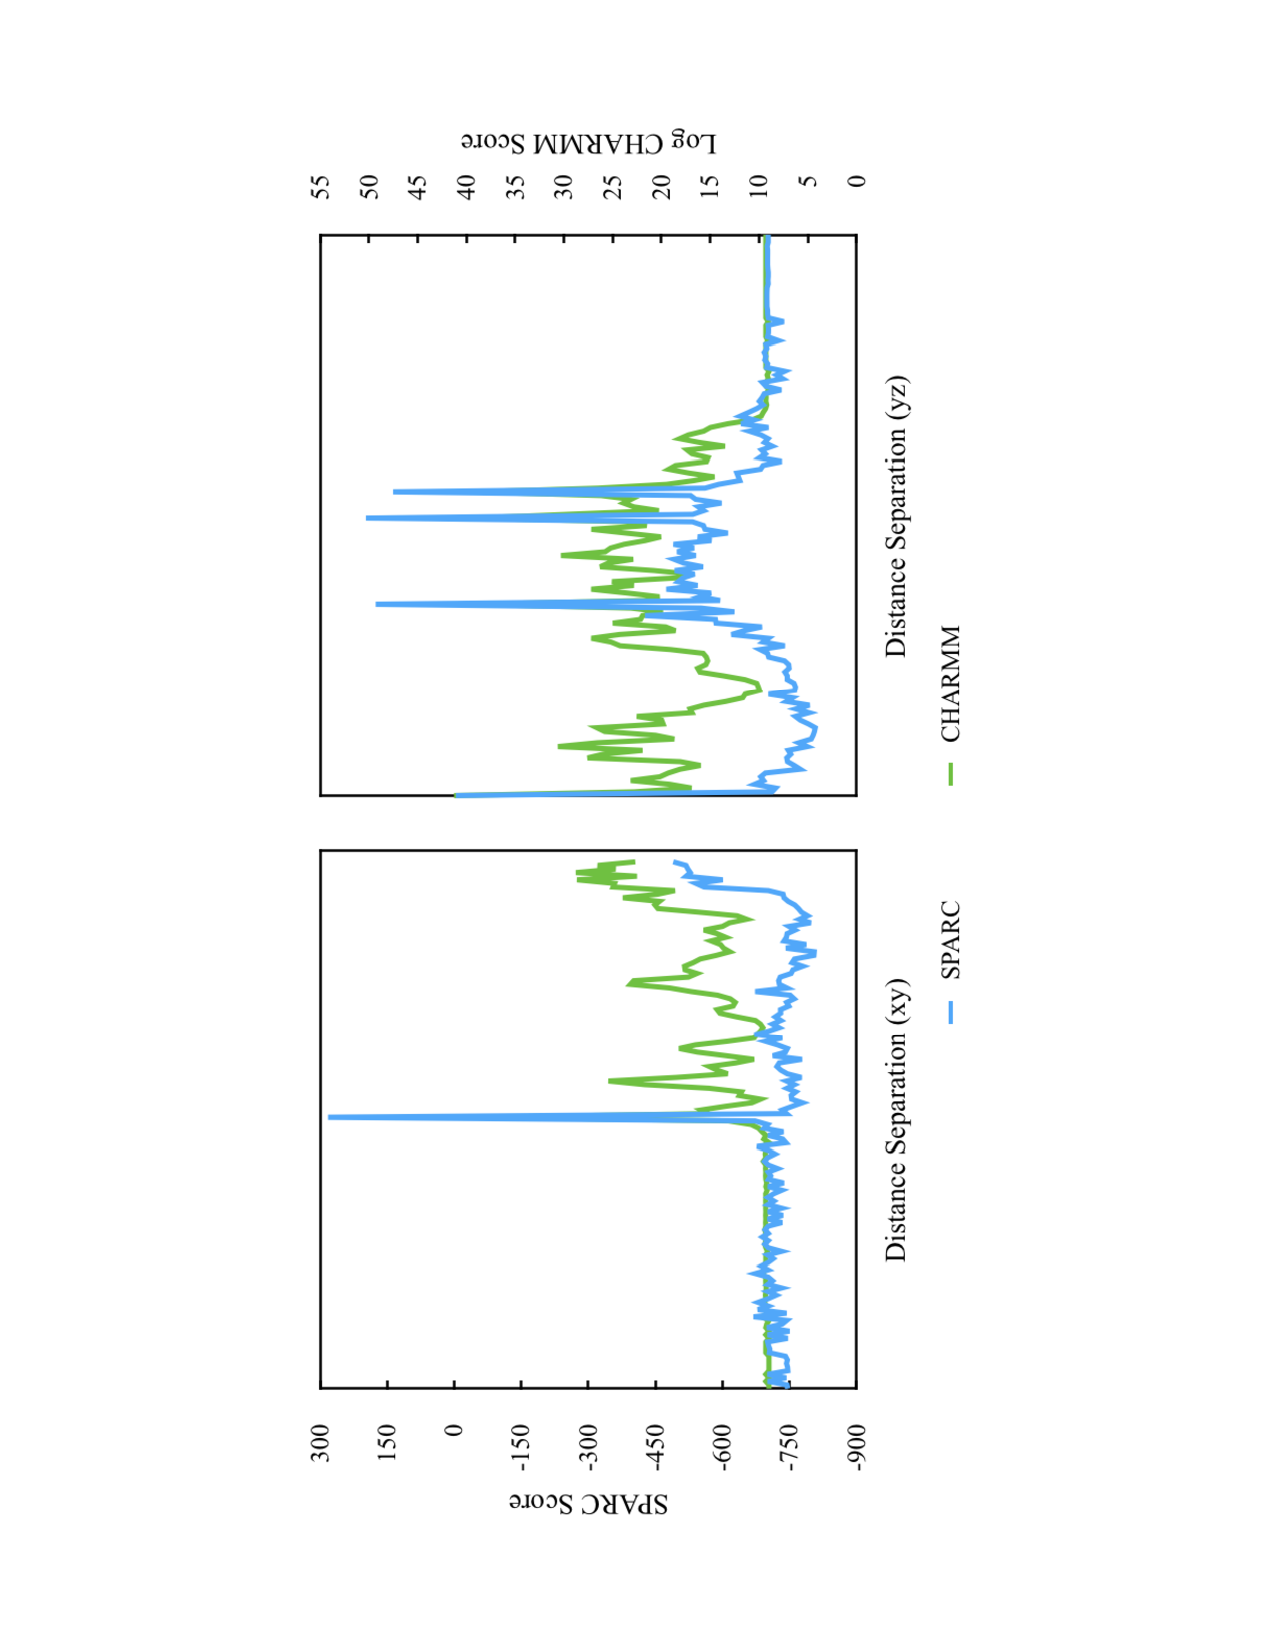
\includegraphics[height=0.9\textwidth, angle=-90, trim=5cm 0 5cm 3cm]{magainin_graphs}
	\caption{The graphs for various translations of the two helices of the magainin structure. Notably, SPARC mimics the local contours of the potential curve even though the absolute energy values do not show a strong correlation. (The distance values are not shown because they are irregular, due to the energy minimization performed before evaluation.)}
	\label{magainin_graphs}
\end{figure}

\subsection{Evaluation with gapless threading}
The most common way to assess the discriminating ability of a statistical potential is through its performance on the gapless threading problem: to identify the most stable conformation out of an ensemble of ``decoy'' structures onto which the same amino acid sequence is threaded.
These databases vary considerably in difficulty, so SPARC was tested on decoy sets from the Decoys 'R' Us database \cite{samudrala} as well as the I-TASSER Decoy Set II \cite{zhang}.

In Table \ref{decoy_table}, we present the results of this test alongside the published statistics of other statistical potentials.
GOAP \cite{zhou2} is an anisotropic potential that uses a conceptually similar approach to SPARC but with orientations determined by heavy atoms in each residue.
(The potential developed by Buchete et al. \cite{buchete2003,buchete3} is coarse-grained like SPARC, but the numerical accuracies on these decoy sets were not given in the original publication.)
For comparison with non-orientational methods we include DFIRE, an all-atom distance-dependent potential that utilizes a distance-scaled ideal gas reference state.
Overall, SPARC achieved an accuracy of 68\%, compared to 48.9\% by DFIRE and 80.1\% by GOAP.

Because the energylike quantities obtained from Eqs. (\ref{sparc_equation}) and (\ref{solvent_equation}) are obtained differently and cannot simply be added together, a weighting procedure was performed to determine the optimum linear combination of the three energy terms (consecutive, nonconsecutive, and solvent).
The integer weights that yielded the highest number of correct native structures was 4 for consecutive, 9 for nonconsecutive, and 3 for solvent interactions.

\begin{table}
	\begin{center}
	\begin{tabular}{c c c c c}
		\toprule
		Decoy Set & \# Decoys & DFIRE & GOAP & SPARC \\
		\midrule
		4state\_reduced & 7 & 6 (-3.48) & 7 (-4.38) & 6 (-4.06)  \\
		fisa\_casp3 & 5 & 4 (-4.8)  & 5 (-5.27)  & 3 (-3.60)  \\
		lmsd & 10 & 7 (-0.88) & 7 (-4.07) & 5 (0.52)   \\
		lattice\_ssfit & 8 & 8 (-9.44) & 8 (-8.38) & 7 (-4.04)  \\
		hg\_structal & 29 & 12 (-1.97) & 22 (-2.73) & 18 (-1.74) \\
		ig\_structal & 61 & 0 (0.92)   & 47 (-1.62) & 33 (-1.60) \\
		I-TASSER & 56 & 49 (-4.02) & 45 (-5.36) & 48 (-7.44) \\
		\midrule
		Total & 176 & 86 & 141 & 120 \\
		\bottomrule
	\end{tabular}
	\end{center}
	\caption{SPARC was tested on the gapless threading problem, which entails predicting the native structure out of an ensemble of decoys ``threaded'' with the same structure. The decoy sets vary in size and difficulty, but overall SPARC was superior in accuracy to the distance-dependent DFIRE potential (data obtained from \cite{zhou2}) and slightly inferior to GOAP, an all-atom orientation-based potential. The numbers given in parentheses are Z-scores for the native structure; more negative values are better.}
	\label{decoy_table}
\end{table}

In addition to the standard decoy tests, the CASP11 decoy set was used to test the correlation between the root-mean-square deviation (RMSD) from the native structure and the SPARC energy score.
RMSD is calculated from two protein structures \textbf{x} and \textbf{y} as $\sqrt{\frac{1}{n}\sum_{i=1}^{n}||\textbf{x}_i - \textbf{y}_i||^2}$ over the $\alpha$-carbons in each structure, and serves as a measure of the difference between the structures.
In Fig. \ref{rms_graphs}, two characteristic RMSD graphs are shown for the CASP11 decoys.

\begin{figure}
	\begin{center}
	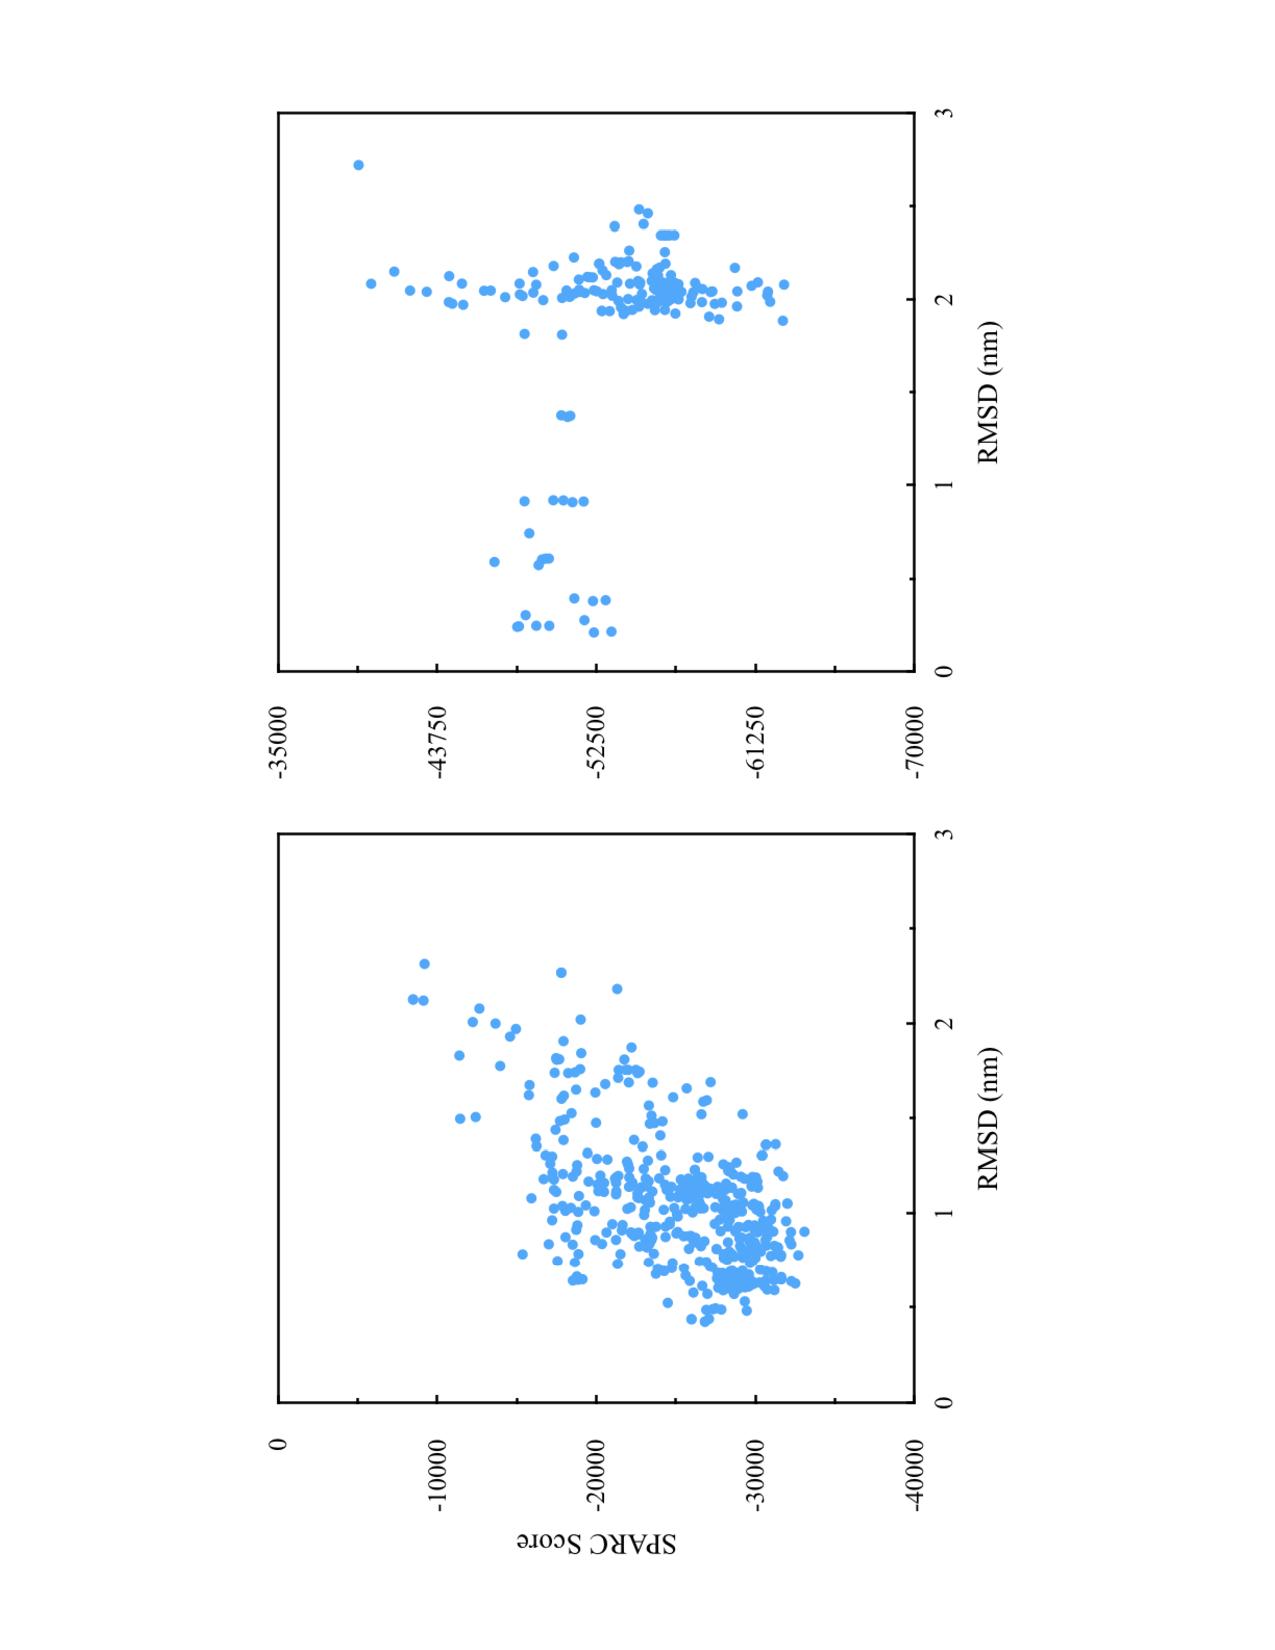
\includegraphics[height=0.8\textwidth, angle=-90, trim=5cm 0 5cm 0]{rmsd_graph}
	\end{center}
	\caption{Two illustrative root-mean-square deviation (RMSD) graphs from the CASP11 set. In the left graph (PDB 2MQ8), there is a clear correlation between the RMSD and the energy score. However, in the right graph (PDB 4Q5T), a conformation cluster at around RMSD = 2 nm appears more stable than the native structure. See Discussion.}
	\label{rms_graphs}
\end{figure}

\subsection{Simulation of a small globular protein}
Using the weighted potential terms from the decoy set results, we applied SPARC to \textit{ab initio} protein structure prediction.
Bovine pancreatic trypsin inhibitor (BPTI, PDB code 1QLQ), a 58-amino acid protein, was chosen for this study because of its simple structure (two $\alpha$-helices and a pair of antiparallel $\beta$-strands) and because it is conventional for testing protein structure prediction algorithms.

First, the effect of manipulating the segment length $\ell$ was tested on the BPTI structure by running 500 iterations at segment lengths from 1--5.
The average, minimum, and variance of the energy scores are given in Table \ref{segment_length_table}.
The mean energy over the course of the simulation increases sharply at $\ell=4$, and while the minimum is not affected, the variance shows a stark increase until $\ell=5$.

\begin{table}
	\begin{center}
		\begin{tabular}{c c c c c c}
			\toprule
			Segment Length & 1 & 2 & 3 & 4 & 5 \\
			\midrule
			Mean     & -93.38  & -93.52  & -93.84  & -89.68  & -90.08  \\
			Minimum  & -136.60 & -123.77 & -129.88 & -132.45 & -140.87 \\
			Variance & 159.57  & 174.75  & 209.01  & 499.12  & 303.67 \\ 
			\bottomrule
		\end{tabular}
	\end{center}
	\caption{Statistics on the energy scores given by SPARC over 500 iterations of the simulation algorithm at various segment lengths. Until $\ell=4$, the variance monotonically increases, suggesting that grouping amino acids together leads to more erratic simulation.}
	\label{segment_length_table}
\end{table}

In accordance with this increase in variance with increasing segment length, a random selector was designed to choose a certain value of $\ell$ with a weight proportional to

\begin{equation}
-\frac{1}{9}\left(x-e^{\frac{4}{225}S+2}\right)^2+4,
\end{equation}

which favors slightly greater segment lengths when the potential energy score $S$ is high.
In addition, the behavior of the simulation was split into two modes, dubbed ``erratic'' and ``gentle''; the erratic mode helps prevent the simulation from being trapped in local energy minima, and the gentle mode refines the structure to cultivate more stable interactions.

Over 2,000 iterations, the SPARC energy scores followed the curve shown in Fig. \ref{simulation_scores}. 
The result closest to the native structure in terms of RMSD was found at the 1,278th iteration with a score of -106.4 and RMSD 8.78 \AA\,, compared to -140.9 for the native structure.
As intended, the ``erratic'' and ``gentle'' modes produced markedly different energy patterns; gentle groups of iterations were relatively inflexible and tended to decrease the energy scores slightly, while erratic iterations were more chaotic (average variance 60.0 compared to 365.6).

\begin{figure}
	\begin{center}
		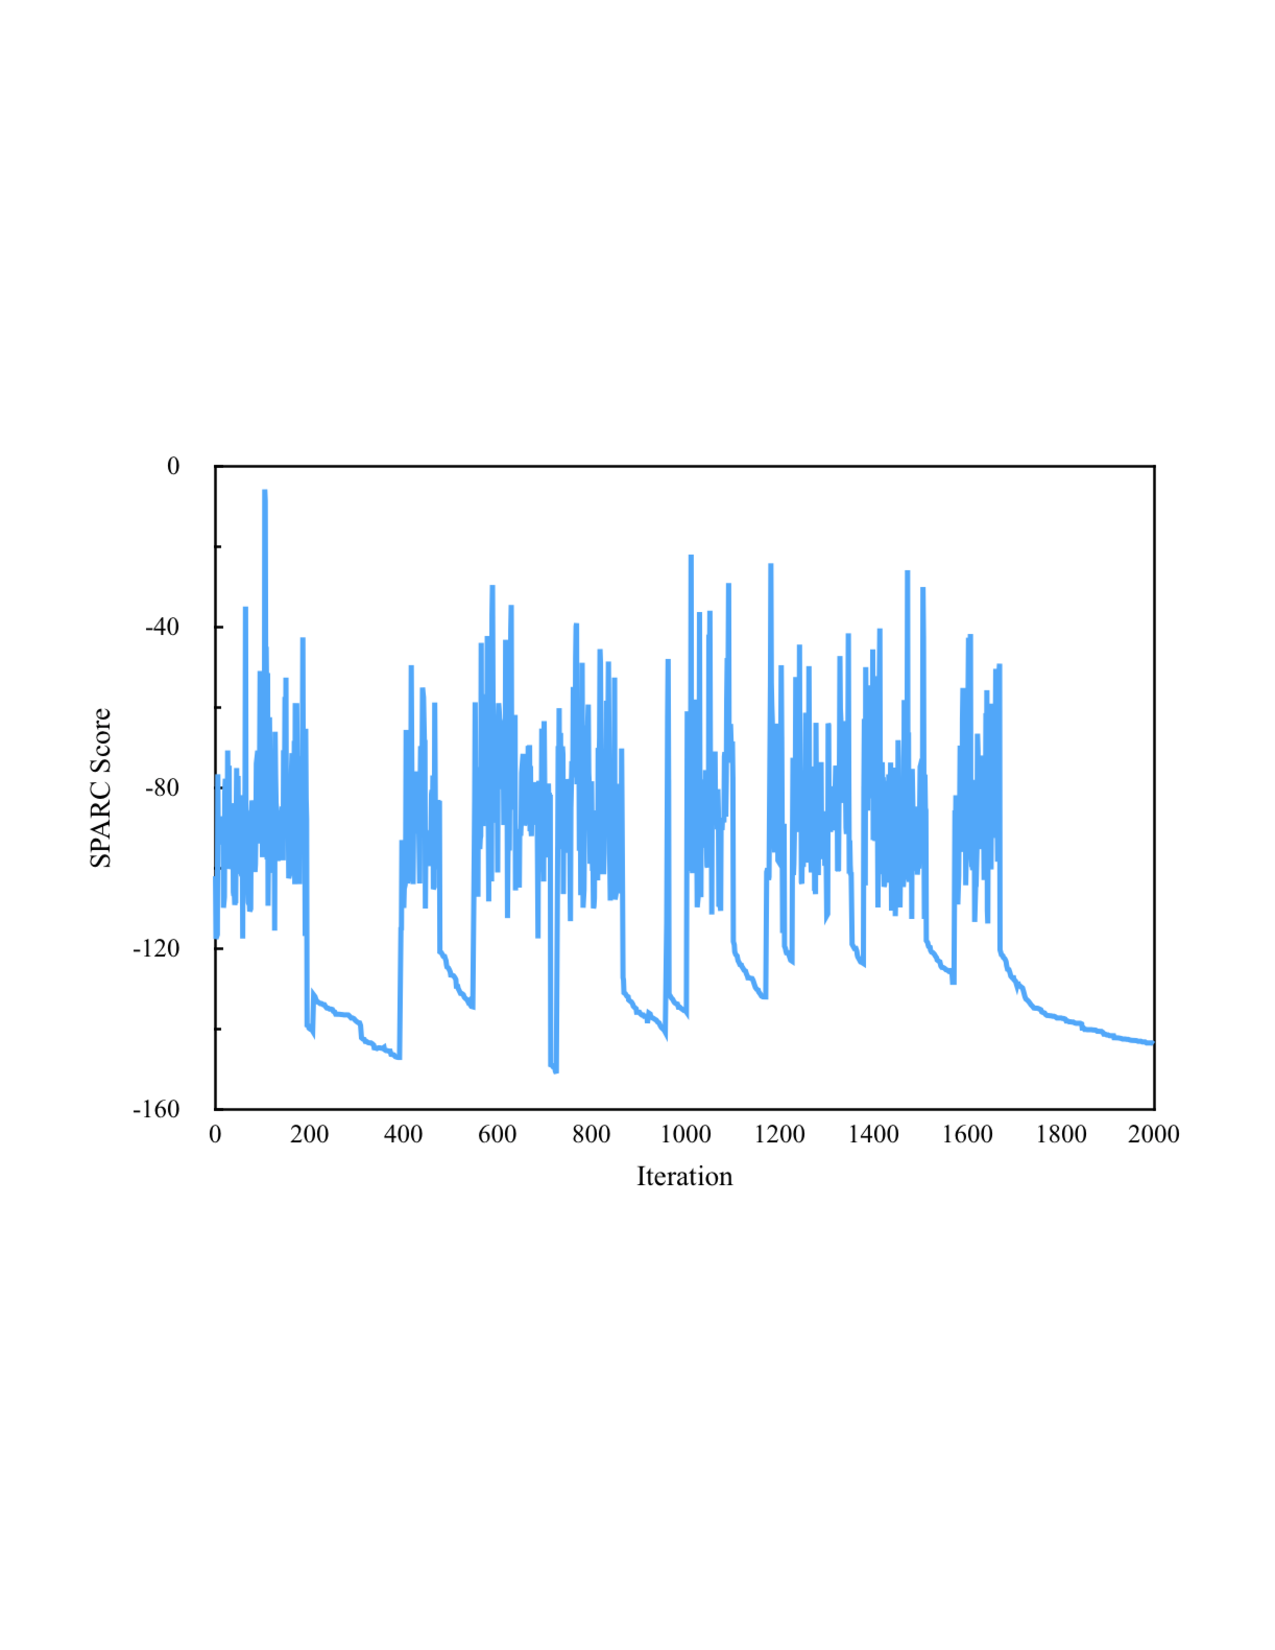
\includegraphics[width=0.8\textwidth, trim=0 7cm 0 7cm, clip=true]{simulation_scores}
	\end{center}
	\caption{SPARC energy scores over the course of a short simulation of bovine pancreatic trypsin inhibitor (BPTI) folding. The steady, deep regions correspond to ``gentle'' mutations, while the rapidly fluctuating iterations are ``erratic'' and designed to introduce variability into the structure.}
	\label{simulation_scores}
\end{figure}

\begin{figure}
	\begin{center}
		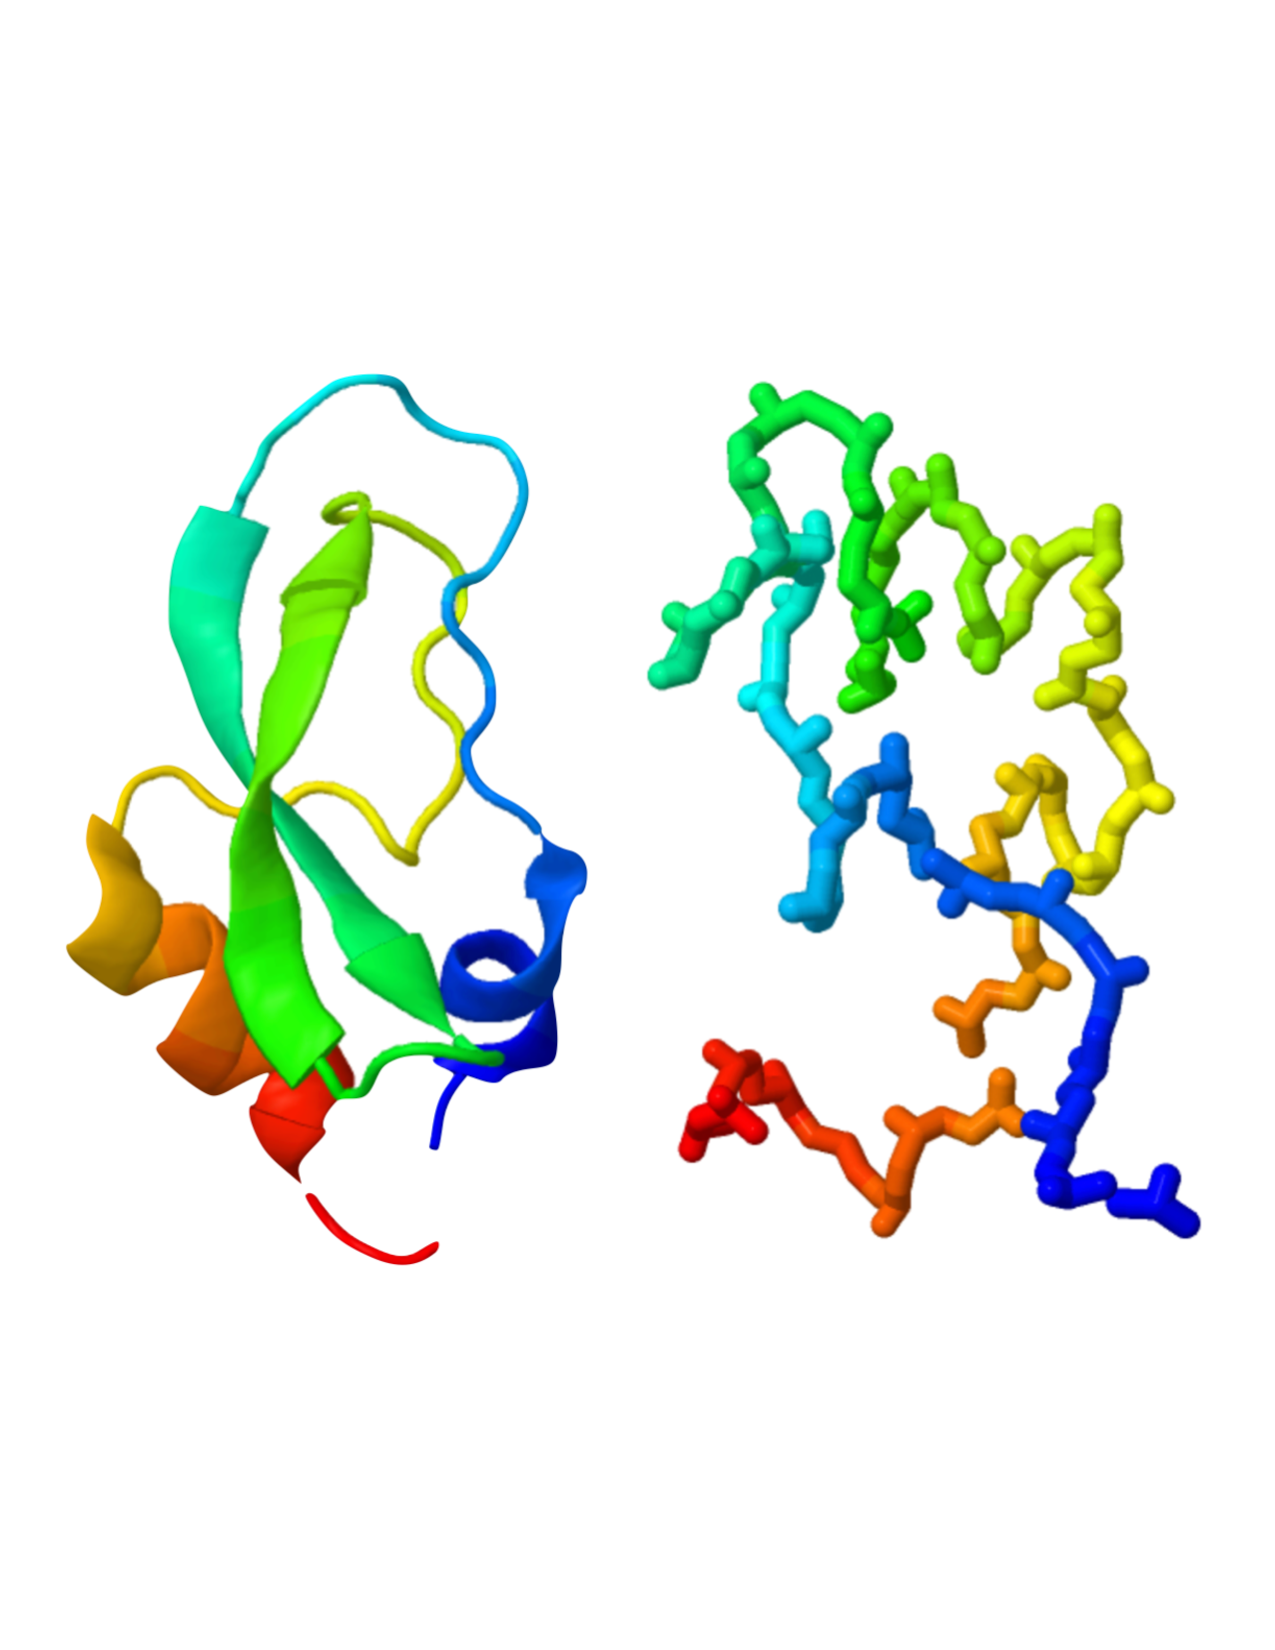
\includegraphics[width=0.6\textwidth, trim=0 5.5cm 0 5.5cm, clip=true]{bpti_structures}
	\end{center}
	\caption{Comparison of the native structure of BPTI (left) with the closest structure predicted by SPARC and the Monte Carlo simulation (right, RMSD = 8.78\AA). There are clear differences in the predicted conformation, but the beginnings of secondary structure and the formation of contacts can be seen.}
	\label{bpti_structures}
\end{figure}

\section{Discussion}
Unlike other statistical potentials, SPARC utilizes a combination of orientational inter-residue interactions and coordination number-based solvent interactions to thoroughly describe the energy of a protein.
When designing a coarse-grained approach to any algorithmic task, it is important to minimize the loss in accuracy over the improvement in performance.
Current potentials range from all-atom \cite{basdevant} to solely contact-based \cite{buchete2}, but SPARC uniquely captures the orientational stability without losing the performance of a coarse-grained method.

SPARC runs quickly once the distributions are calculated, but the construction of the potential itself was extremely time-consuming, taking roughly two weeks to compute all of the relative orientations in the 91,995-structure sample on the two machines.
The additional time spent analyzing this dataset (which is an order of magnitude larger than the sets used for most other potentials) improved the potential's resolution, since it better differentiated the low-frequency bins.
The correlations between CHARMM and SPARC on the magainin test did show some lack of definition for CHARMM energies greater than $10^{20}$ kcal/mol, but these extremely high values would be rare in a simulation.
One major change that would improve the accuracy of SPARC, at the expense of performance, would be to combine the relative orientations in each LCS as they occurred in the native ensemble.
As Eq. (\ref{sparc_equation}) shows, the frequencies from each residue's LCS are added independently, when in reality certain orientations are likely to be conditional to specific orientations of the other residue.
We did not implement this change because it would effectively have squared the potential tables' memory requirement; however, it could be an area for extension in a future version.

The comparison of CHARMM and SPARC using the magainin protein illustrates a clear correspondence between the scores given by each potential.
Given the diversity of the terms which compose an all-atom potential, it is remarkable that the solely statistical SPARC model is able to approximate the contours of the CHARMM energy function.
The gapless threading test illustrated a similar trend, but here in comparison to more similar knowledge-based methods.
DFIRE, a distance-dependent potential, was less effective than either of the two anisotropic potentials, confirming that distance alone is not sufficient to describe the energy of a protein.
(The same was found in the test with magainin, where distances varied in different directions resulted in different energy curves.)
GOAP, which is based on orientations of heavy atoms within each amino acid as well as atomic distances, has a higher accuracy than SPARC, most likely because of its all-atom components.
Since SPARC does not consider the exact locations of atoms within each residue, only the VSEPR-derived Cartesian coordinates, it cannot distinguish between structures with stable sidechains and those with infeasible packing arrangements.
For our potential to perform better on the gapless threading test, we could add additional terms to describe the sidechain arrangements.
However, our Monte Carlo simulation algorithm, designed for SPARC, circumvents this issue by checking for steric violations at every iteration and allowing only permissible consecutive orientations.

Although the simulations we performed were relatively short, they are representative of the characteristic of the algorithm since the output does not depend on previous iterations.
The energy scores fluctuated frequently because new, unstable structures were introduced by the mutation system.
We did find that mutating longer segments led to more chaotic simulations and greater variance in energy scores, which is most likely a consequence of the restriction to permissible orientations.
Since the mutation in each iteration was cascaded through the chain in either direction to maintain chain connectivity (see Fig. \ref{flowchart}), longer segments led to larger deviations in each cascade.

The experiments with segment length, as well as other tests, allowed us to probabilistically control the introduction of variation into the structure.
In the dynamically-adjusted simulation of BPTI, the energy scores become much steadier and the conformation is conserved to a greater extent when the algorithm recognizes it as being stable.
However, because this simulation is not in physical time, it is appropriate that eventually the mutations interrupt the ``gentle'' iterations to experiment with other shapes.
For instance, the native structure of BPTI gave a SPARC energy score of -140.9, and for 258 points in the run the score dropped below -140.
However, the closest structure in terms of RMSD did not have a comparable energy score (-106.4), which suggests a lack of stabilizing contacts and appropriate secondary structures.
The lowest-energy structures on the other hand, display tighter helices and even some $\beta$-sheets.
We believe that in a longer simulation, even better conformations would appear and be refined, approaching the shape of the native structure and producing even better local orientations than the experimentally-determined BPTI structure.

In summary, the various assessments of SPARC's accuracy suggest a definite set of strengths and weaknesses. 
SPARC is most effective at scoring structures on a macroscopic level, such as the interaction energies between the chains of the magainin protein.
It also proved useful for generating stable local conformations through secondary structure in the BPTI simulation; the greater weight on nonconsecutive interactions also encourages these contacts.
The shortcoming of SPARC is that it is coarse-grained to the residue level, which is an issue if the decoy set or simulation algorithm does not account for steric clashes within the residues.
(This could have also explained why the CHARMM and SPARC energy values did not significantly correlate for the magainin protein.)
The end result is that SPARC and our simulation algorithm yield accurate relative assessments of structures, and with brief deterministic or fine-grained methods these assessments can be improved even further.

\section{Conclusion}
The statistical potential developed in this paper, Segmented Positional Analysis of Residue Contacts (SPARC), contains innovations in several aspects. 
It is based on relative orientations using Cartesian local coordinate system transformations, which describe the protein structure more thoroughly than contact-based or distance-based representations.
On the other hand, SPARC is coarse-grained, which permits it better performance at a small price in accuracy, at least on the gapless threading problem.
SPARC was shown to replicate the contours of the energy function given by a conventional all-atom physics-based force field, and the packing density criterion correlates with a well-known hydrophobicity scale.
Furthermore, the development of an off-lattice simulation algorithm using a novel segmentation technique proved useful for generating realistic candidate conformations in only two thousand iterations.

Using these simulation techniques and potential functions, biologists will be able to model a host of protein activities, including ligand docking, signal transduction, and nucleic acid manipulations\footnote{Nucleic acids are not currently supported by SPARC, but could be easily added with a large enough dataset of nucleotide-amino acid interactions and a simple Python subclass.}.
In addition, this simulation algorithm could be be applied to protein design, which seeks to create protein sequences that have certain structural properties for drug design and gene therapy.
In the future, we are considering expanding SPARC to take advantage of its flexible solvent model in non-aqueous simulations, especially in the plasma membrane where the solvent varies through the environment.
With these adaptations, we hope to develop this orientational approach to protein structure prediction into a general research tool for modeling biomolecular systems.

\bibliographystyle{abbrv}
%\nocite{*}
{\footnotesize \bibliography{biblio.bib}}
\end{document}
